% \documentclass[12pt]{article}
% \begin{document}
\documentclass[aspectratio=169, 11pt]{beamer}
\usepackage{tikz}
\usetheme{Copenhagen}
\usecolortheme{beaver}

\usepackage{booktabs}
\usepackage{graphicx}
\graphicspath{ {img/} }

\begin{document}
\title{Project 2}   
\author{
B03902003 Chia-sheng Chen\\
B03902036 Yen-ting Liu\\
B03902104 Yi-ying Chao} 
\date{\today} 
\frame{\titlepage}

\frame{\frametitle{Table of contents}\tableofcontents} 

\section{L1 Cache}
\subsection{L1 Cache Structure}
\begin{frame}
  \frametitle{System Block Diagram}
  \includegraphics[width=\textwidth]{systemBlockDiagram}\\
  \footnotesize{\# From TA}
\end{frame}

\begin{frame}
  \frametitle{L1 Cache Structure}
  \includegraphics{cacheStructure}
\end{frame}


\subsection{Read and Write of Cache}
\begin{frame}
  \frametitle{Example of Read and Write Structure}
  \includegraphics[height=0.85\textheight]{readWrite}
\end{frame}

\begin{frame}
  \frametitle{Difference}
  \begin{itemize}
  \item 8 Mux instead of 4 Mux when write (8 words in a cache line)
  \item 31:10 tag bit, 9:5 index bit, 4:0 offset bit (spec) 
  \end{itemize}
\end{frame}

\begin{frame}
  \frametitle{Deciding the Source of Data}
  \begin{table}[]
  \centering
  \caption{Deciding the Source of Data}
  \label{my-label}
  \begin{tabular}{@{}lll@{}}
  \toprule
             & Load Word (Read)     & Store Word (Write)                 \\ \midrule
  Cache  Hit & Every word from SRAM & One word from CPU, other from SRAM \\
  Cache Miss & Every word from DRAM & One word from CPU, other from DRAM \\ \bottomrule
  \end{tabular}
  \end{table}
\end{frame}

\tiny
\subsection{Inside Cache Controller}
\begin{frame}
  \frametitle{Finite State Machine}

\begin{center}
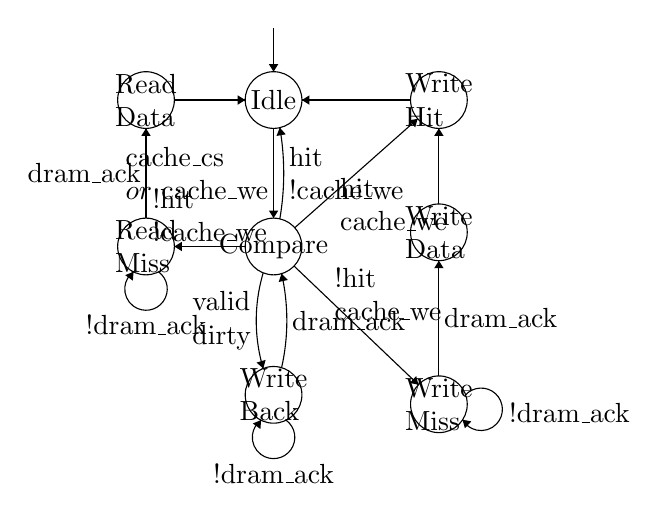
\begin{tikzpicture}[scale=0.12]
\tikzstyle{every node}+=[inner sep=0pt]
\draw [black] (33.1,-9.2) circle (3);
\draw (33.1,-9.2) node {Idle};
\draw [black] (33.1,-24.7) circle (3);
\draw (33.1,-24.7) node {Compare};
\draw [black] (19.6,-24.7) circle (3);
\draw (19.6,-24.7) node [align=left] {Read\\Miss};
\draw [black] (19.6,-9.2) circle (3);
\draw (19.6,-9.2) node [align=left] {Read\\Data};
\draw [black] (33.1,-40.4) circle (3);
\draw (33.1,-40.4) node [align=left] {Write\\Back};
\draw [black] (50.6,-41.4) circle (3);
\draw (50.6,-41.4) node [align=left] {Write\\Miss};
\draw [black] (50.6,-9.2) circle (3);
\draw (50.6,-9.2) node [align=left] {Write\\Hit};
\draw [black] (50.6,-23.2) circle (3);
\draw (50.6,-23.2) node [align=left] {Write\\Data};
\draw [black] (33.1,-1.6) -- (33.1,-6.2);
\fill [black] (33.1,-6.2) -- (33.6,-5.4) -- (32.6,-5.4);
\draw [black] (33.764,-12.124) arc (9.77504:-9.77504:28.424);
\fill [black] (33.76,-12.12) -- (33.41,-13) -- (34.39,-12.83);
\draw (34.68,-16.95) node [right, align=left] {hit\\!cache\_we};
\draw [black] (33.1,-12.2) -- (33.1,-21.7);
\fill [black] (33.1,-21.7) -- (33.6,-20.9) -- (32.6,-20.9);
\draw (32.6,-16.95) node [left, align=left] {cache\_cs\\$or$ cache\_we};
\draw [black] (30.1,-24.7) -- (22.6,-24.7);
\fill [black] (22.6,-24.7) -- (23.4,-25.2) -- (23.4,-24.2);
\draw (26.35,-24.2) node [above, align=left] {!hit\\!cache\_we};
\draw [black] (19.6,-21.7) -- (19.6,-12.2);
\fill [black] (19.6,-12.2) -- (19.1,-13) -- (20.1,-13);
\draw (19.1,-16.95) node [left] {dram\_ack};
\draw [black] (22.6,-9.2) -- (30.1,-9.2);
\fill [black] (30.1,-9.2) -- (29.3,-8.7) -- (29.3,-9.7);
\draw [black] (32.005,-37.611) arc (-163.41994:-196.58006:17.735);
\fill [black] (32.01,-37.61) -- (32.26,-36.7) -- (31.3,-36.99);
\draw (30.77,-32.55) node [left, align=left] {valid\\dirty};
\draw [black] (35.27,-26.77) -- (48.43,-39.33);
\fill [black] (48.43,-39.33) -- (48.2,-38.41) -- (47.51,-39.14);
\draw (45.22,-32.57) node [above, align=left] {!hit\\cache\_we};
\draw [black] (50.6,-38.4) -- (50.6,-26.2);
\fill [black] (50.6,-26.2) -- (50.1,-27) -- (51.1,-27);
\draw (51.1,-32.3) node [right] {dram\_ack};
\draw [black] (50.6,-20.2) -- (50.6,-12.2);
\fill [black] (50.6,-12.2) -- (50.1,-13) -- (51.1,-13);
\draw [black] (35.35,-22.71) -- (48.35,-11.19);
\fill [black] (48.35,-11.19) -- (47.42,-11.35) -- (48.09,-12.09);
\draw (45.81,-17.44) node [below, align=left] {hit\\cache\_we};
\draw [black] (47.6,-9.2) -- (36.1,-9.2);
\fill [black] (36.1,-9.2) -- (36.9,-9.7) -- (36.9,-8.7);
\draw [black] (53.418,-40.405) arc (137.17202:-150.82798:2.25);
\draw (57.97,-42.33) node [right] {!dram\_ack};
\fill [black] (53.1,-43.03) -- (53.35,-43.94) -- (54.03,-43.21);
\draw [black] (34.423,-43.08) arc (54:-234:2.25);
\draw (33.1,-47.65) node [below] {!dram\_ack};
\fill [black] (31.78,-43.08) -- (30.9,-43.43) -- (31.71,-44.02);
\draw [black] (20.923,-27.38) arc (54:-234:2.25);
\draw (19.6,-31.95) node [below] {!dram\_ack};
\fill [black] (18.28,-27.38) -- (17.4,-27.73) -- (18.21,-28.32);
\draw [black] (33.952,-27.574) arc (12.71147:-12.71147:22.613);
\fill [black] (33.95,-27.57) -- (33.64,-28.46) -- (34.62,-28.24);
\draw (35.01,-32.55) node [right] {dram\_ack};
\end{tikzpicture}
\end{center}
\end{frame}
\end{document}

